\chapter{Introducing Rainbow Trout}

\section{Trout Species}

There are 206 species in the family of {\it Salmonidae}. 
Salmonids (salmon, trout, char and whitefish) are found in practically all continents, 
partly because they are indigenous there and partly because they have been introduced.

Among trout, brook trout, brown trout, lake trout, sea trout and rainbow trout are the most 
widely known species.

\subsection{Brown Trout} 

Brown Trout are native to Europe and West Asia. An important market and sport fish, 
it has been introduced to many different countries all over the world, see figure  ~\ref{fig:BrownTrout}


\begin{figure}[H]
  \centering
   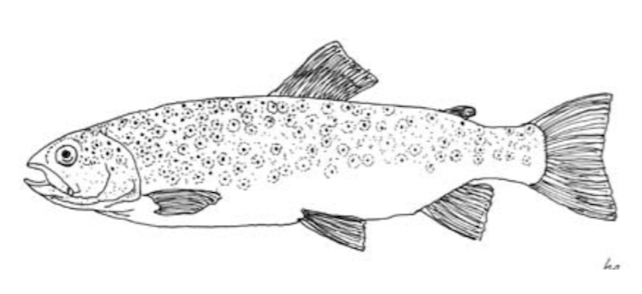
\includegraphics[scale = 0.5]{images/BrownTrout.png}
  \caption{Brown Trout.}
   \label{fig:BrownTrout}
\end{figure}

According to their habitat, taxonomists distinguish three forms of Brown Trout. 
They are the actual brown trout {\it Salmo trutta m. fario},  the
lake trout {\it Salmo trutta m. lacustris} and sea trout {\it Salmo trutta m. trutta},



\subsection{Brook Trout}

Brook Trout, together with Lake Trout {\it Salvelinus namaycush}, belongs to the {\it char} 
subgroup of salmonids, which distinguishes it from trout and salmon, see figure  ~\ref{fig:BrookTrout}

\begin{figure}[H]
  \centering
   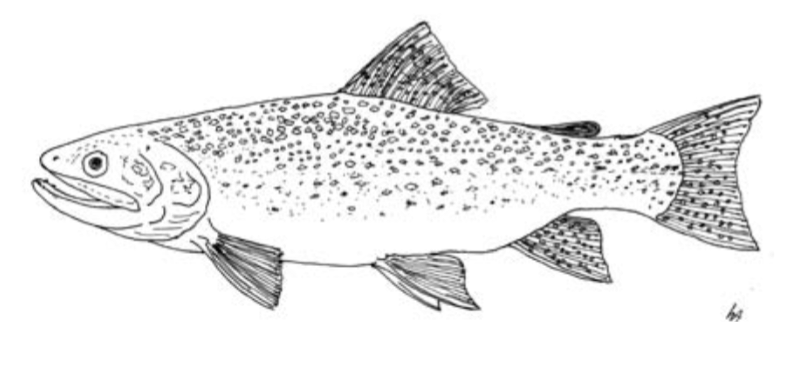
\includegraphics[scale = 0.5]{images/BrookTrout.png}
  \caption{Brook Trout.}
   \label{fig:BrookTrout}
\end{figure}

The Brook Trout is one of the most well-known sport fish and is native to the northeast of the United States of America and the east region of Canada. It has been introduced to many countries of South America, Oceania and Asia, and to practically all of the countries of Europe and the former Soviet Union.


\subsection{Rainbow Trout} 

Rainbow Trout, {\it Oncorhynchus mykiss}, is a highly commercial sport and market fish.
A normal adult rainbow trout weighs about 2-3 kg, while its maximum size, weight and age are 120 cm total length (TL), 25.4 kg and 11 years, respectively. Rainbow Trout live in the upper, cold water sections of rivers and seas, see figure  ~\ref{fig:RainbowTrout}

\begin{figure}[H]
  \centering
   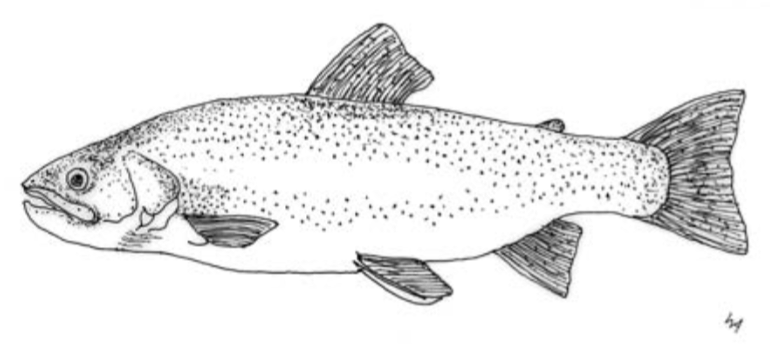
\includegraphics[scale = 0.5]{images/RainbowTrout.png}
  \caption{Rainbow Trout.}
   \label{fig:RainbowTrout}
\end{figure}

As in the case of other trout, the habitat and food of rainbow trout determine both their actual colour and shape.
The Rainbow Trout has many local strains, which have developed in the different river systems. Out of these, numerous improved commercial strains have been bred. The widely cultured commercial strains have been improved from those original rainbow trout populations that possessed advantageous qualities, such as hardiness, fast growth, resistance to diseases and reliable reproduction under farm conditions.


\section{Rainbow Trout in the Wild}

In the wild, there are rainbow trout populations that spawn in autumn and there are other populations that spawn in spring. From these populations, two different commercial strains have been bred. Their qualities are similar, only their spawning seasons differ from each other. This enables the production capacities of a rainbow trout farm to be increased.

\subsection{Habitat}
There are many habitat factors that basically influence the growth of rainbow trout. These include basic water qualities and the abundance of natural food.

A Rainbow trout is a typical cold water fish see the optimal temperature ranges in figure  ~\ref{fig:TempRanges}

\begin{figure}[H]
  \centering
   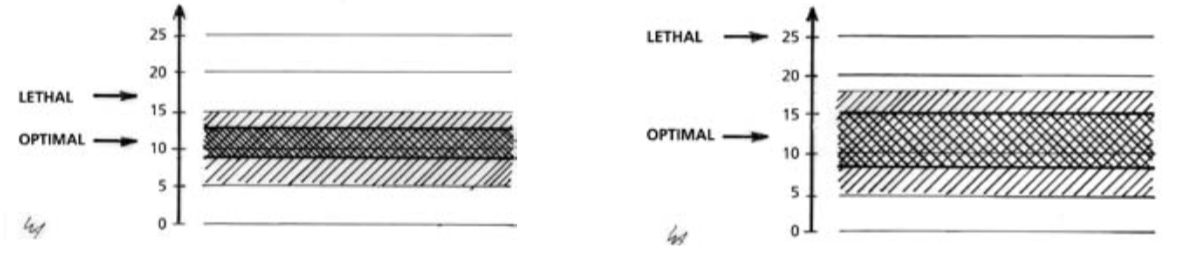
\includegraphics[scale = 0.7]{images/TempRanges.png}
  \caption{Optimal Temperature ranges for Rainbow Trout at different development stages: {\bf left:} during the incubation of eggs and sac fry, {\bf right:} during the growth. }
   \label{fig:TempRanges}
\end{figure}

Apart from temperature the other factors that influence growth are:

\begin{itemize}
\item[]Clear water: Keen eyesight is crucial for efficient feeding.
\item[]Dissolved oxygen: Water should sustain dissolved oxygen (DO) in high concentrations, in order to ensure smooth respiration. 
\item[]Clean water: Water should be free of harmful solid and gaseous waste materials produced during metabolism and respiration.
\end{itemize}


\subsection{Natural food} The natural food of rainbow trout depends on the age and size of fish, on the size of food item and on the habitat occupied. Rainbow trout are aggressive and greedy in feeding. They are opportunistic feeders that grab and eat almost anything. Figure ~\ref{fig:NaturalFood} summarises the most frequent natural food items of rainbow trout.


\begin{figure}[H]
  \centering
   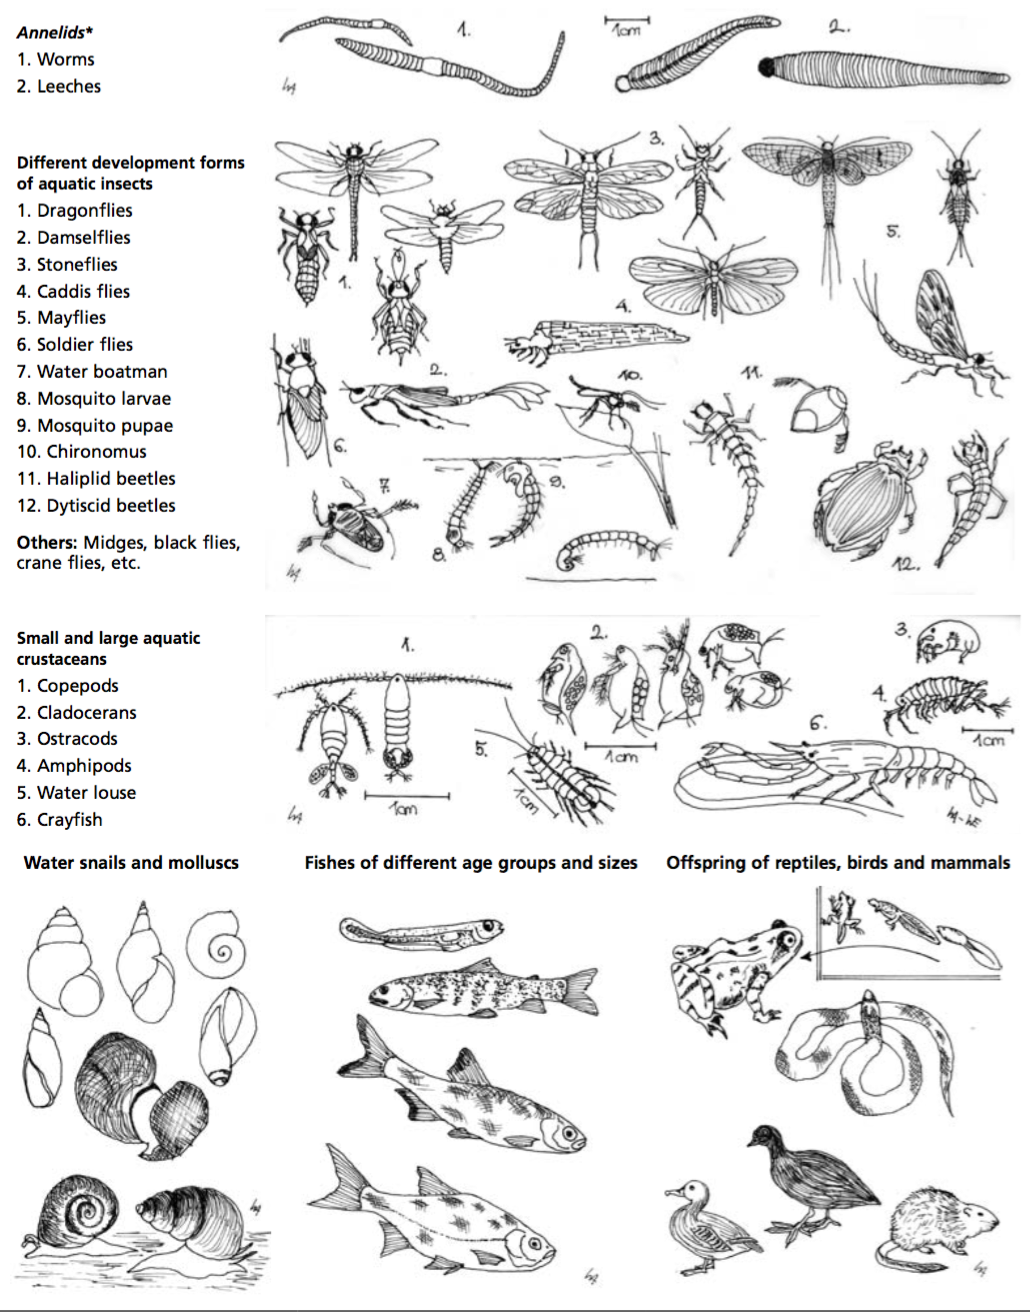
\includegraphics[scale = 0.5]{images/NaturalFood.png}
  \caption{Natural Food Sources for Rainbow Trout.}
   \label{fig:NaturalFood}
\end{figure}

Terrestrial insects are also consumed when they fall into the water. These insects are adult beetles {\it Coleoptera}, flies {\it Diptera}, ants {\it Formicidae} and larvae of moths and butterflies, {\it Lepidoptera}. 

\subsection{Life Cycle and Development Phases}

\begin{figure}[H]
  \centering
   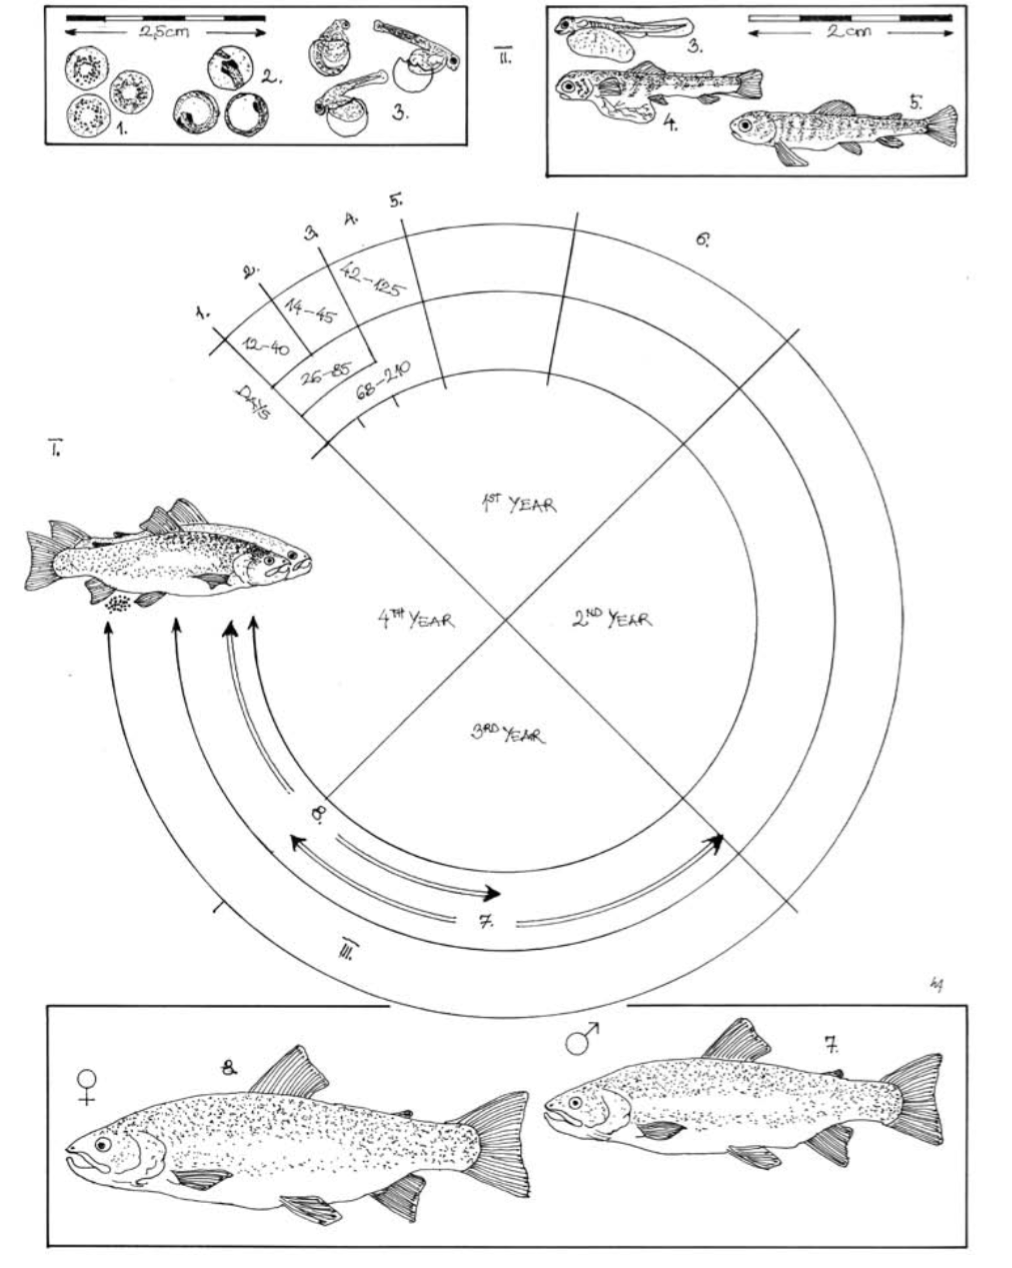
\includegraphics[scale = 0.6]{images/LifeCycle.png}
  \caption{Rainbow Trout Development Stages: 
  1. Fertilized eggs. 2. Eyed egg. 3. Hatched sac fry. 4. Swim-up fry. 5. Fry. 
6. One-summer fish. 7. Sexually mature male and 8. female ready to spawn}
   \label{fig:LifeCycle}
\end{figure}

Figure ~\ref{fig:LifeCycle} shows the life cycle and development stages for rainbow trout in the wild.
The actual start and duration of the different development phases depend on the water temperature, 
the genotype as well as the quantity and quality of available natural fish food.

\subsection{Body Parts}

Figure ~\ref{fig:BodyParts} and ~\ref{fig:LengthMeasurements} shows the body parts of a rainbow trout and the standard length measurements.



\begin{figure}[H]
  \centering
   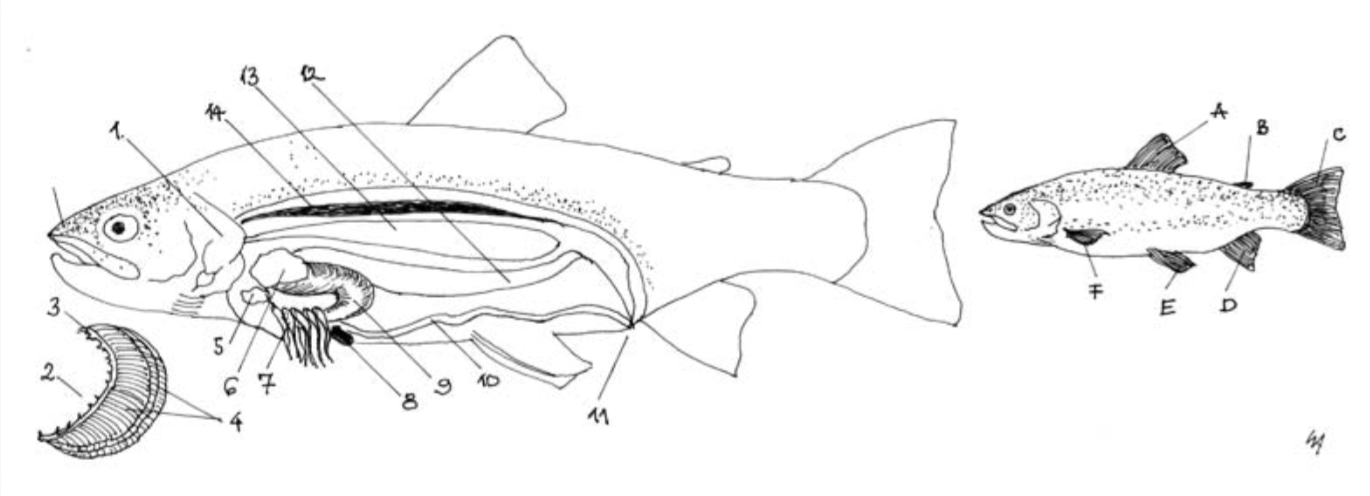
\includegraphics[scale = 0.5]{images/BodyParts.png}
    \caption{Rainbow Trout Body Parts: 
  1. Opercula (gill cover). 2. Gill raker. 3. Gill arch. 4. Gill filaments. 5. Heart. 6. Liver. 7. Pyloric caecae and pancreas. 8. Spleen. 9. Stomach. 10. Intestine. 11. Anus and urogenital papilla. 12. Gonad. 13. Swimming bladder. 14. Kidney. A. Dorsal fin. B. Adipose fin. C. Caudal fin. D. Anal fin. E. Pelvic fin. F. Pectoral fin.}
   \label{fig:BodyParts}
\end{figure}

\begin{figure}[H]
  \centering
   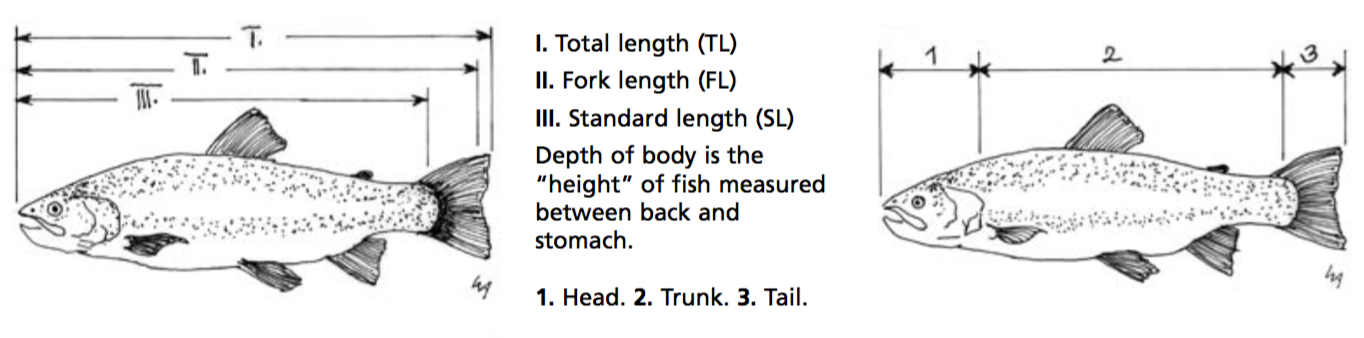
\includegraphics[scale = 0.6]{images/LengthMeasurements.png}
    \caption{Rainbow Trout Standard Length Measurements.}
   \label{fig:LengthMeasurements}
\end{figure}


\subsection{Length versus Weight}

Figure ~\ref{fig:LengthWeight} shows the correlation between its total length and weight.

\begin{figure}[H]
   \centering
   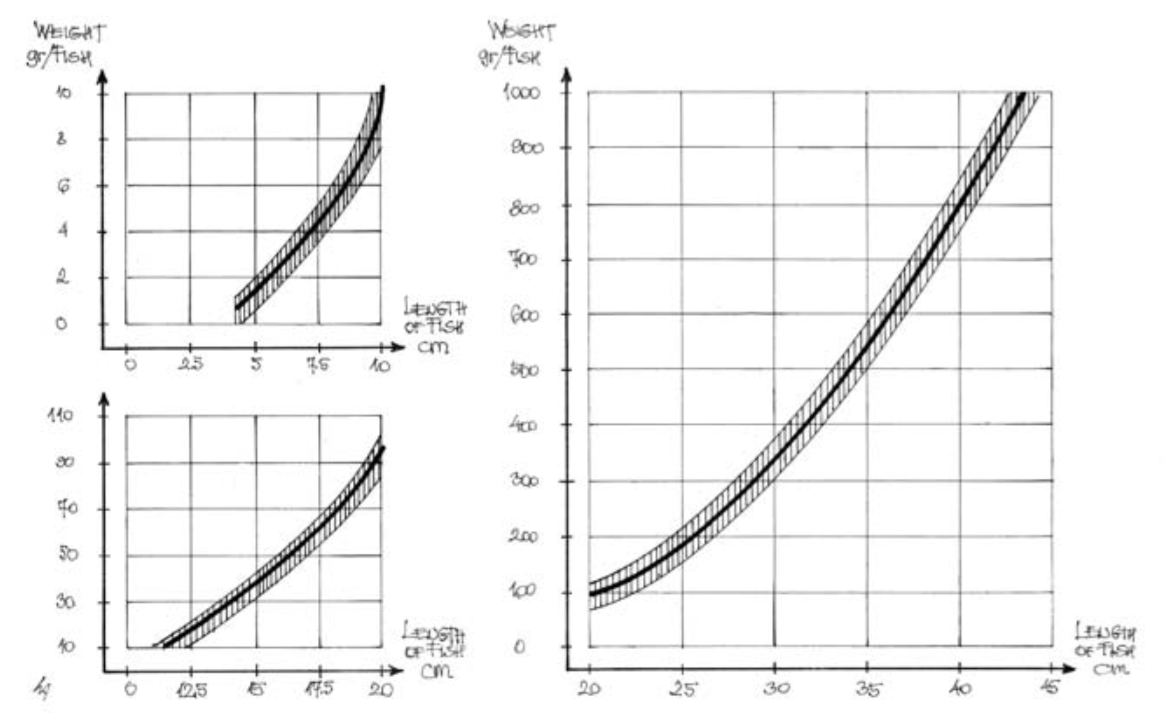
\includegraphics[scale = 0.6]{images/LengthWeight.png}
    \caption{Rainbow Trout Standard Length versus Weight Correllations.}
   \label{fig:LengthWeight}
\end{figure}

\subsection{Duration of development stages}

Water temperature is a major determining factor of fish production. 
This is because the body temperature of embryos, fry and developing fish equalise 
their temperature to that of the water they are in. 
Along with the body temperature, the intensity of the metabolism also changes.

The developing embryos and fry feed from the yolk sac and receive oxygen through the entire body surface. When the water temperature is higher, the embryos and fry develop more rapidly, while at lower water temperatures the speed of development reduces. Outside of a certain range of water temperature development stops.

\begin{figure}[H]
   \centering
   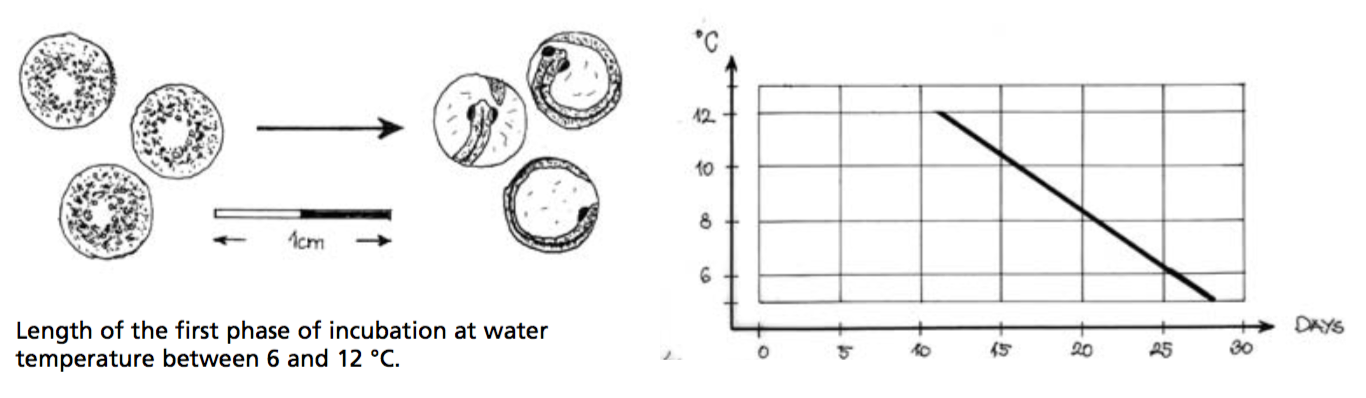
\includegraphics[scale = 0.6]{images/DurationIncubationFirstPhase.png}
    \caption{Duration of First Phase of Incubation.}
   \label{fig:DurationIncubationFirstPhase}
\end{figure}

\begin{figure}[H]
   \centering
   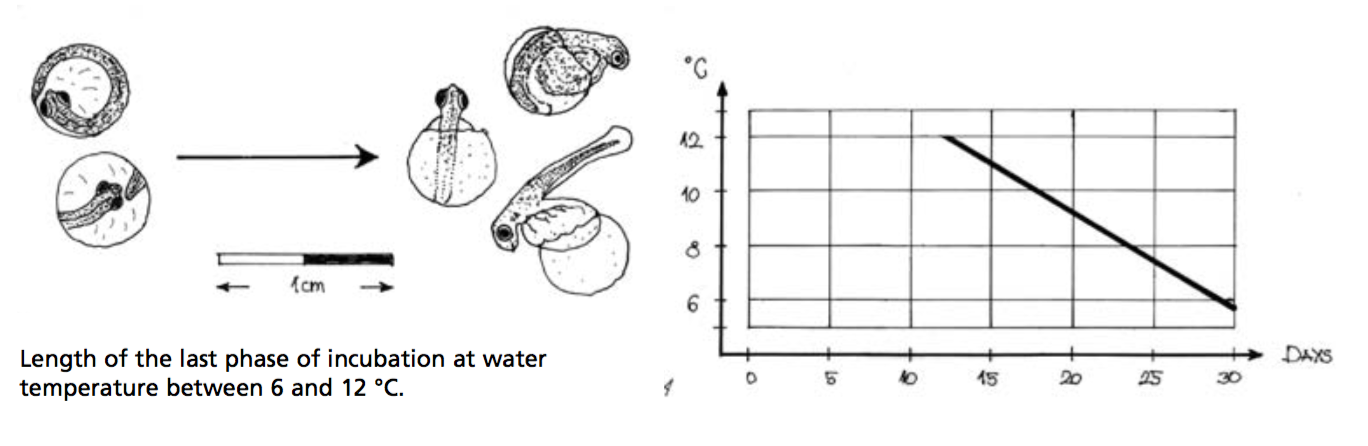
\includegraphics[scale = 0.6]{images/DurationIncubationLastPhase.png}
    \caption{Duration of Last Phase of Incubation.}
   \label{fig:DurationIncubationLastPhase}
\end{figure}

\begin{figure}[H]
   \centering
   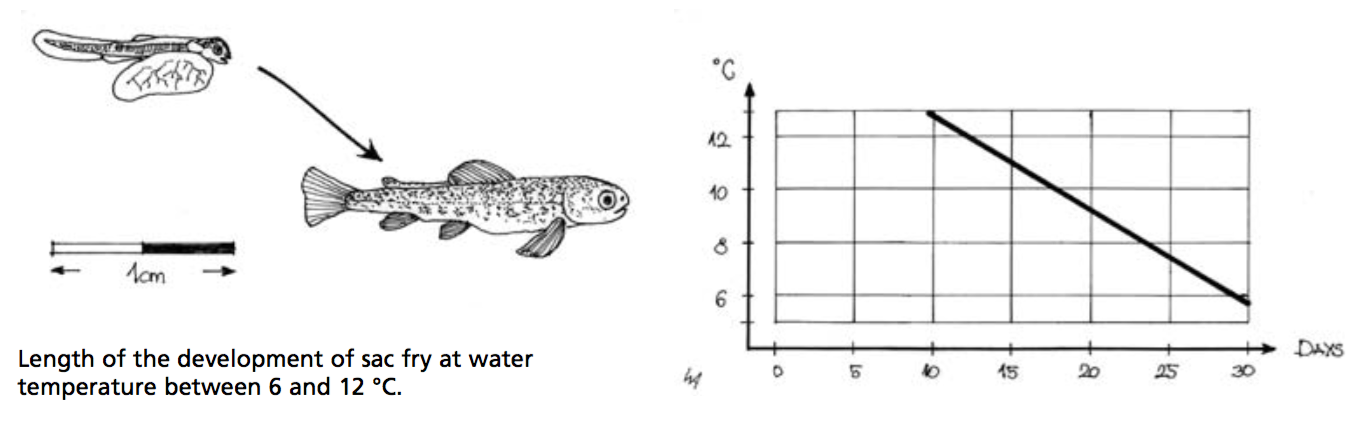
\includegraphics[scale = 0.6]{images/DurationSacFry.png}
    \caption{Duration of Sac Fry Development.}
   \label{fig:DurationSacFry}
\end{figure}

The total length of the development of embryo and fry from fertilisation to swim-up is about 37-83 days at water temperatures between  \SI{6}{\celsius} and  \SI{12}{\celsius}.

After starting external feeding, the actual length of the development of the different age groups depends not only on the temperature and oxygen content of water but also on the quality and quantity of consumed feed. Here, it has been assumed that trout is adequately fed with commercial feeds. 

Development of fry from swim-up fry takes 1.5-3 months, see figure ~\ref{fig:DurationSacFry}. Here. {\it fry} refers to a total length of 5 cm and to an average body weight of 2 g.

\begin{figure}[H]
   \centering
   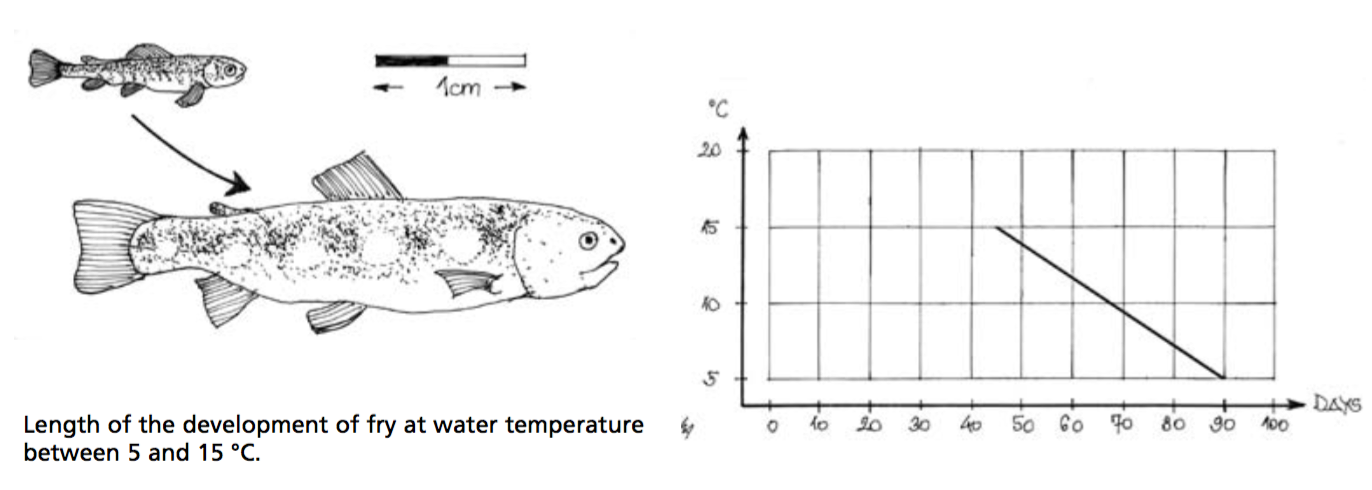
\includegraphics[scale = 0.6]{images/DurationFry.png}
    \caption{Duration of Fry Development.}
   \label{fig:DurationFry}
\end{figure}

Development of fingerlings from fry takes 3-4.5 months, see figure ~\ref{fig:DurationFry}. Here, {\it fingerling} refers to a total length of 12.5 cm and to an average body weight of 25 grams.

\begin{figure}[H]
   \centering
   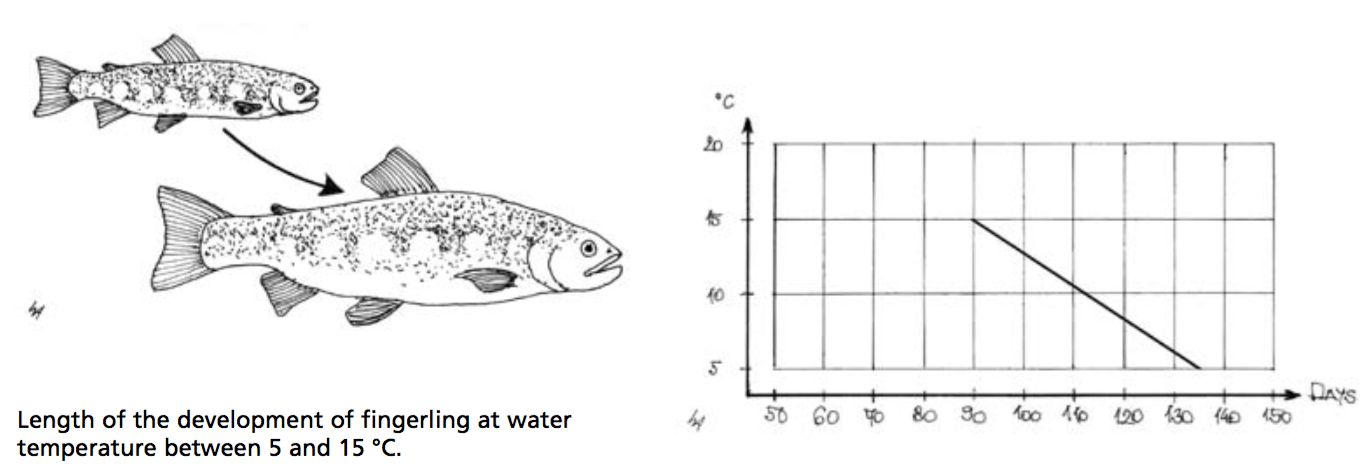
\includegraphics[scale = 0.6]{images/DurationFingerlings.png}
    \caption{Duration of Fingerling Development.}
   \label{fig:DurationFingerlings}
\end{figure}

Development of table fish from fingerling takes 4-6.5 months,  see figure ~\ref{fig:DurationFingerlings} . Here, {\it table fish} refers to the desired minimum body weight of 250 g.

\begin{figure}[H]
   \centering
   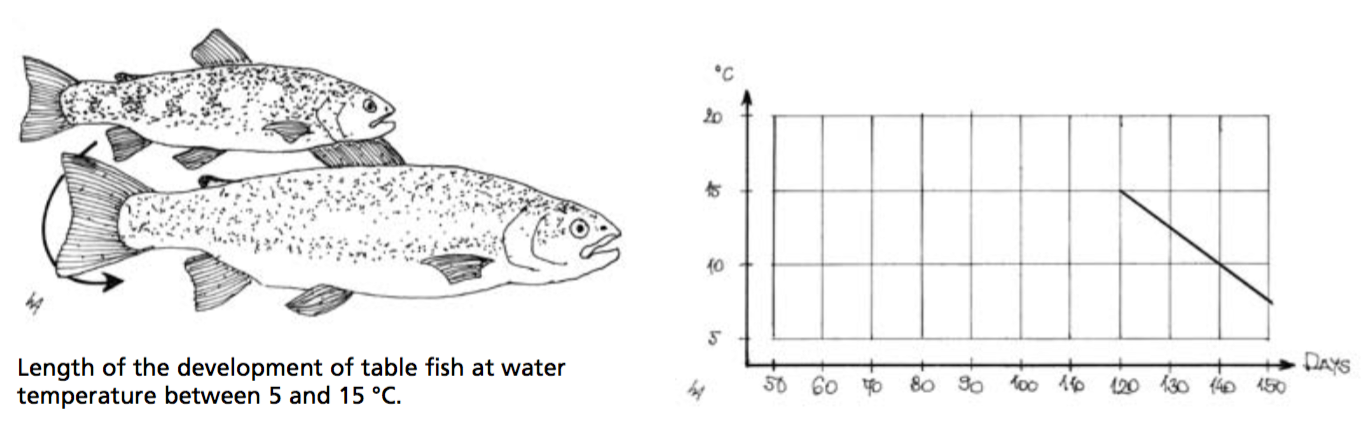
\includegraphics[scale = 0.6]{images/DurationTableFish.png}
    \caption{Duration of Table Fish Development.}
   \label{fig:DurationTableFish}
\end{figure}

Growth of large table fish from 250 g to 500 g takes a further 2.5-4.5 months (75-135 days) when the water temperature is between  \SI{5}{\celsius} and  \SI{15}{\celsius}.



\section{Production Conditions}

In this section we outline the optimal or near to optimal conditions that should be ensured during production of the different age stages of Rainbow Trout. 

\subsection{Water pH} 

Rainbow Trout tolerates unfavourable pH conditions differently during the various development phases of the fish. The optimal and acceptable ranges of pH of rearing water also differ. For developing embryos and fry, the range of optimal pH is narrow, and varies between 6.5 and 8, but the range of acceptable pH is also narrow. For older fish, both the optimal and acceptable ranges of pH are wider, as demonstrated in figure ~\ref{fig:OptimalPH}.

\begin{figure}[H]
  \centering
   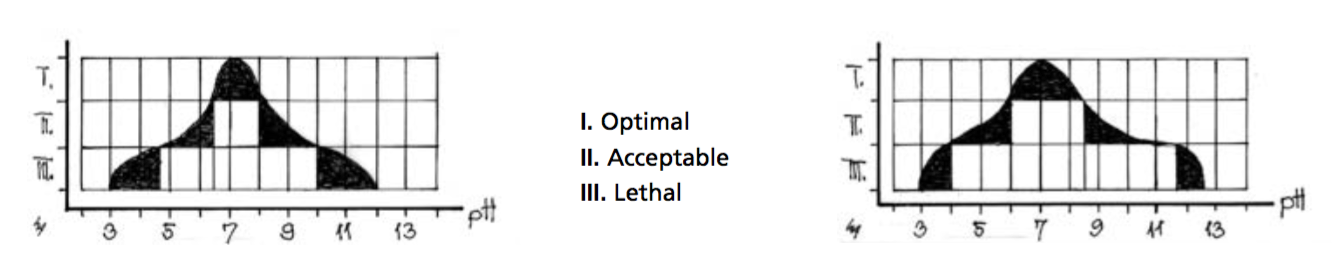
\includegraphics[scale = 0.5]{images/OptimalPH.png}
  \caption{Optimal pH ranges for embryos and swim-up fry on the left and growing fish on the right.}
   \label{fig:OptimalPH}
\end{figure}


\subsection{Water Temperature} 

The optimal, acceptable and lethal ranges of water temperature also vary according to the development stages of the fish, as demonstrated in figure \ref{fig:OptimalTemp}.

\begin{figure}[H]
  \centering
   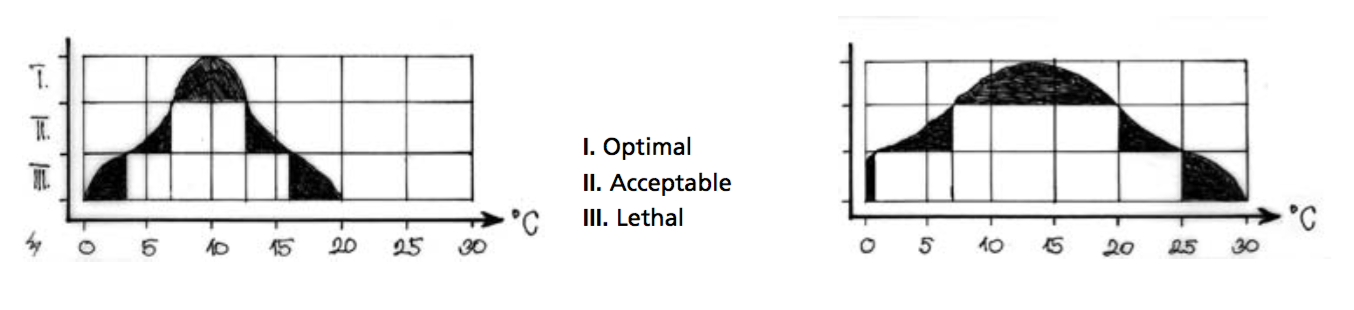
\includegraphics[scale = 0.5]{images/OptimalTemp.png}
  \caption{Optimal temperature ranges for embryos and swim-up fry on the left and growing fish on the right.}
   \label{fig:OptimalTemp}
\end{figure}


There is a range of water temperature, about \SI{7}{\celsius} to \SI{18}{\celsius}, where the appetite of feeding rainbow trout is optimal, see figure \ref{fig:OptimalAppetite}. Outside of this range, at lower and higher water temperature, fish lose appetite. Finally, at too low or too high water temperature, fish stop feeding.

Feed intake of rainbow trout intensifies as the water temperature increases. However, this behaviour continues only up to about \SI{18}{\celsius}.  Above this temperature, the appetite of and feed intake by the fish sharply decreases and stops.

\begin{figure}[H]
  \centering
   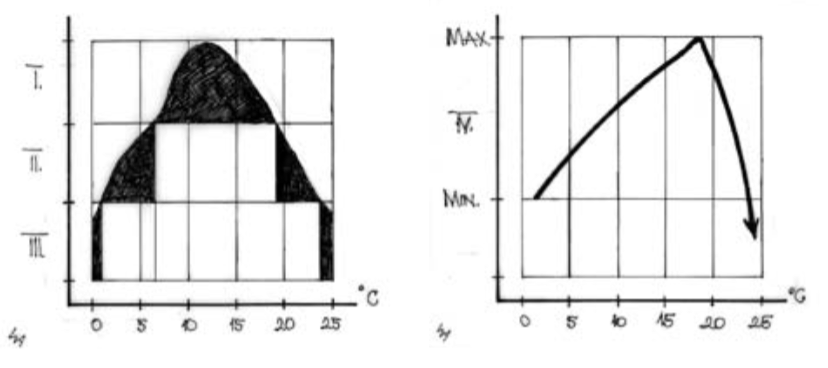
\includegraphics[scale = 0.5]{images/OptimalAppetite.png}
  \caption{ I. Optimal range of appetite. II. Losing appetite. III. Feeding stops. IV. Intensity of feeding..}
   \label{fig:OptimalAppetite}
\end{figure}

It is important to be aware that there is an inverse correlation between the intensity of feeding and the utilisation of consumed feed. Thus, at about \SI{18}{\celsius}, rainbow trout are willing to feed very intensively, but the digestion of consumed feed will be less complete at this temperature. The water temperature where the different trout species make the best growth out of the consumed feed varies from \SI{13}{\celsius} to \SI{15}{ \celsius}. 

\subsection{Water Oxygen Content}

Oxygen dissolved in water ensures the respiration of the different aquatic plants and animals. 
Most frequently, the DO content of water is expressed in milligrams of oxygen per litre of water (mg/litre).
The maximum oxygen content of water depends on the water temperature. 
This is because water can dissolve only a certain quantity of oxygen, which is determined by the partial pressure of oxygen in the atmosphere.
Figure ~\ref{fig:OxygenTemp} shows the inverse correlation between temperature and DO content of water. 
At a higher temperature of water, the DO content is lower. 
At maximum oxygen content, water is 100 percent saturated with oxygen and the oxygen in excess soon leaves to the atmosphere.

\begin{figure}[H]
  \centering
   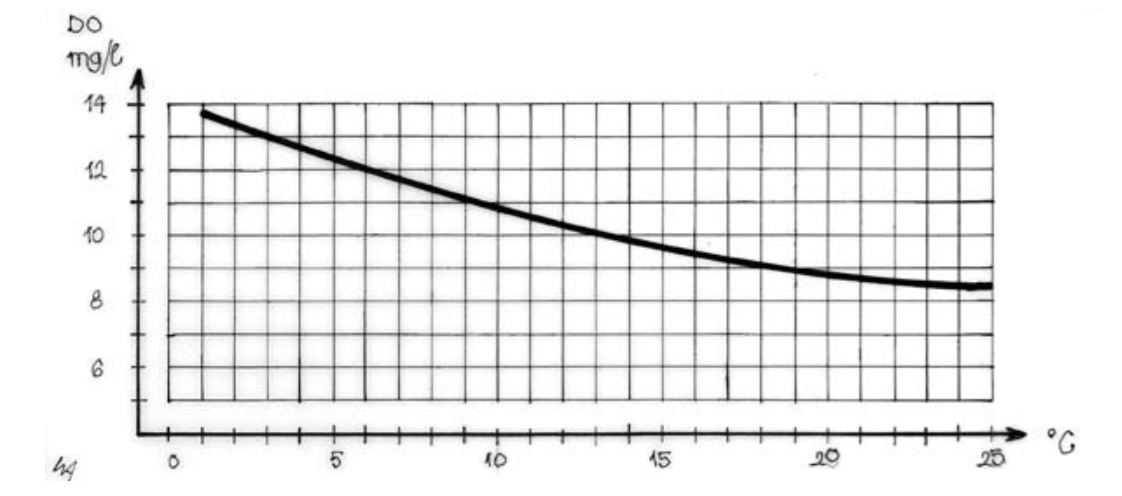
\includegraphics[scale = 0.5]{images/OxygenTemp.png}
  \caption{ Correlation between temperature and maximum oxygen saturation.}
   \label{fig:OxygenTemp}
\end{figure}


The optimal and acceptable concentrations of oxygen in water vary according to the actual development stage of the fish. The optimum is when the oxygen content of rearing water is near to saturation (100 percent). The acceptable range of oxygen content of rearing water is lower. It ranges between 5 and 6 mg/litre during incubation of eggs and the first development stages of fry. For older age groups, the acceptable low oxygen content of water may be about 4.5 mg/litre.

It is important to know that the oxygen consumption of fish increases considerably during and after feeding. During these periods the demand for oxygen will temporarily increase.

\subsection{Water Supply}

In order to ensure the replacement of used water in the rearing devices, a continuous supply of fresh, clean and oxygen-rich water is essential. The necessary quantities of water supplied depend on the age and actual quantity of the developing fish.

The quantity of eggs, fry and growing fish per unit area of rearing device is determined by the oxygen content of supplied water. In colder water, the metabolism and, hence, respiration slows, while in warmer water they intensify. Accordingly, the actual quantity of water needed for the same number of developing embryos, fry and fish will be different. At low water temperature, the quantity of water supplied may be less but at higher water temperature it should be more. See figure ~\ref{fig:WaterSupply} 

\begin{figure}[H]
  \centering
   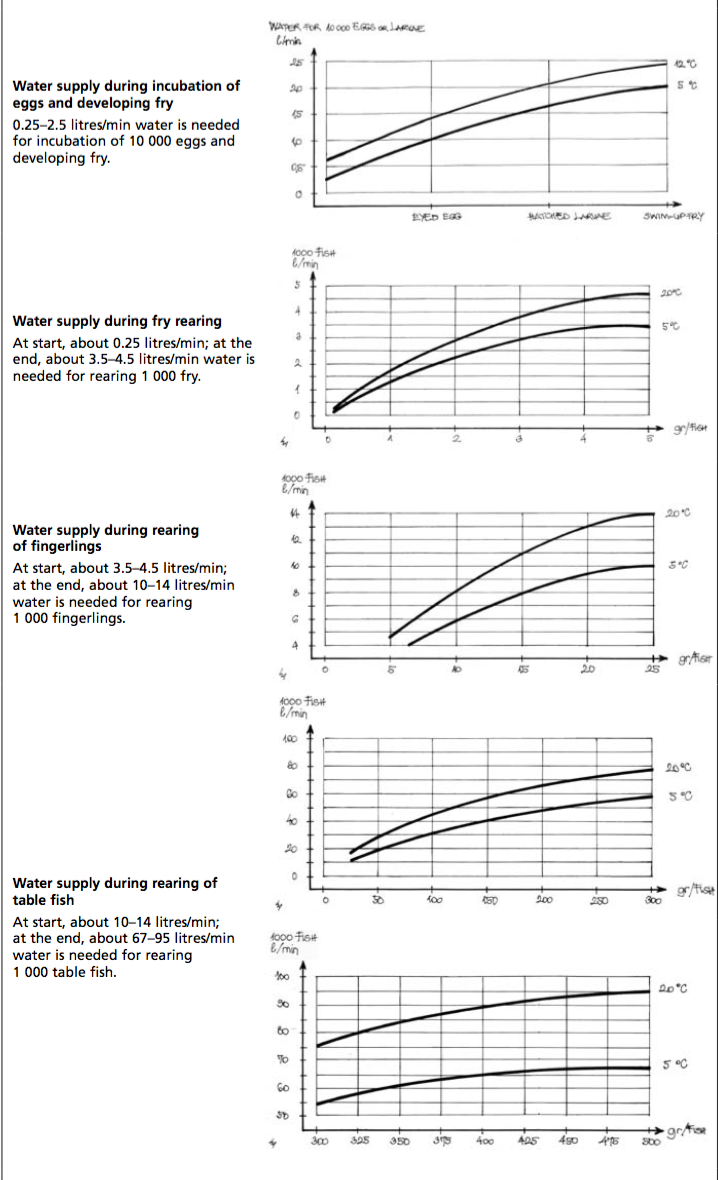
\includegraphics[width=8cm]{images/WaterSupply.png}
  \caption{ Water supply in tanks required according to development stage of fish. }
   \label{fig:WaterSupply}
\end{figure}


Water supply is expressed by the flow rate, which is the quantity of water needed for 10 000 specimens of eggs or 1 000 specimens of fry or fish. It is expressed either in litres per second (litre/s) or litres per minute (litres/min). 

Frequency of water exchange is another way to specify the quantity of supplied water. It is expressed by the exchange rate of water per hour or day.

The water supply in concrete or lined tanks can be more intensive than in earth ponds, hence the density of fish can also be higher in these devices.

\subsection{Aeration Principles}

In the practice of pond fish farming oxygen deficiency has been regarded as dangerous mainly because 
of mass losses of fish. But recent investigations have shown that decreased oxygen saturation can 
have serious effects on the economy of a fish farm as well.

Keeping the dissolved oxygen content of the pond water nearly at the saturation level makes it possible 
not only to avoid mass losses of fish but ensures better conversion rates and higher yields in intensive culture.

Most trout farms use flow-through systems, whereby grow-out tanks are continuously refreshed 
with large quantities of new water, usually gravity-fed from nearby streams or rivers. 
Whether rectangular raceways or self-cleaning circular tanks are employed, 
the essentials remain the same; rapid removal of wastes and 
continuous replenishment of the system with highly oxygenated water.
